%Autor: miguev
%miguev: 15

\chapter{Yacas}
\label{yacas.tex}

\index{Yacas}
\index{cálculo simbólico}

En  este tema  aprenderás a  utilizar el  programa Yacas  para relizar
cálculos simbólicos.  Este tipo de  cálculos resulta de  gran utilidad
puesto que  funciona de  la misma  forma que harías  tú mismo  a mano,
operando con expresiones matemáticas sin calcular el valor numérico de
cada expresión. 



\section{¿Qué es Yacas?}

Yacas  es un  Sistema  de  Álgebra Computacional  (en  inglés CAS,  de
\index{CAS}
\index{Álgebra Computacional}
Computer  Algebra  System) de  propósito  general  fácil de  usar.  Un
Sistema  de Álgebra  Computacional (SAC)  es un  programa que  permite
manipulaciones simbólicas sobre expresiones matemáticas, reduciendo el
tiempo necesario  para realizar  cálculos embarazosos  pero triviales.
Esto se hace  no mediante números, sino mediante símbolos,  por lo que
el resultado de una operación con expresiones matemáticas es una nueva
expresión matemática.

Yacas  está  construido  sobre  su  propio  lenguaje  de  programación
diseñado  para  este  propósito,  en  el  que  se  pueden  implementar
fácilmente  nuevos  algoritmos.  Además, incorpora  una  documentación
extensa sobre las funcionalidades que  implementa y los métodos usados
para implementarlas.

Entre las  características que Yacas implementa  encontramos precisión
arbitraria, números racionales,  vectores, números complejos, cálculos
con  matrices  (incluyendo  inversas, determinantes  y  resolución  de
sistemas lineales), derivación, series  de Taylor, resolución numérica
(método  de Newton),  y un  montón más  de algoritmos  no matemáticos.
Tiene  también  soporte  básico   para  polinomios  en  una  variable,
integración de funciones y cálculo tensorial.

En  la  web  del proyecto  Yacas  ({\tt  http://yacas.sourceforge.net}
encontrarás el  código fuente  del programa  y toda  su documentación:
desde  un tutorial  básico hasta  una guía  de programación  en Yacas.
Parte  del  texto de  este  tema  son  traducciones  de trozos  de  la
documentación oficial de Yacas que se distribuye junto con el programa
bajo licencia GPL.



\section{Empezando con Yacas}

Yacas  tiene  un  intérprete  de comandos  que  nos  permite  ejecutar
funciones para probar  lo que queremos programar,  para luego escribir
un script  (un fichero de  comandos a modo  de guión). Para  entrar al
intérprete de Yacas  basta con ejecutar el comando {\tt  yacas} en una
consola  o terminal.  Para  salir del  intérprete  puedes pulsar  {\tt
Control-C}  o bien  ejecutar la  función \verb+Exit();+.  Pulsar  {\tt
Control-C} también  es útil  para detener inmediatamente  la ejecución
del intérprete de Yacas (o de un script escrito para Yacas).

\begin{verbatim}
$ yacas
[editvi.ys] [unix.ys] 
True;
Numeric mode: "Gmp"
To exit Yacas, enter  Exit(); or quit or Ctrl-c. Type ?? for help.
Or type ?function for help on a function.
Type 'restart' to restart Yacas.
To see example commands, keep typing Example();
In>
\end{verbatim}

También  existe una  interfaz gráfica  llamada Proteus.  Si la  tienes
instalada  deberías   poder  iniciarla  ejecutando  el   comando  {\tt
proteusworksheet}. Esta utilidad te proporciona un entorno  más cómodo
e integrado  en el  que  puedes  probar código  en  el intérprete e ir
escribiendo un script en el editor que incluye.

\begin{figure}[hbt]
\centering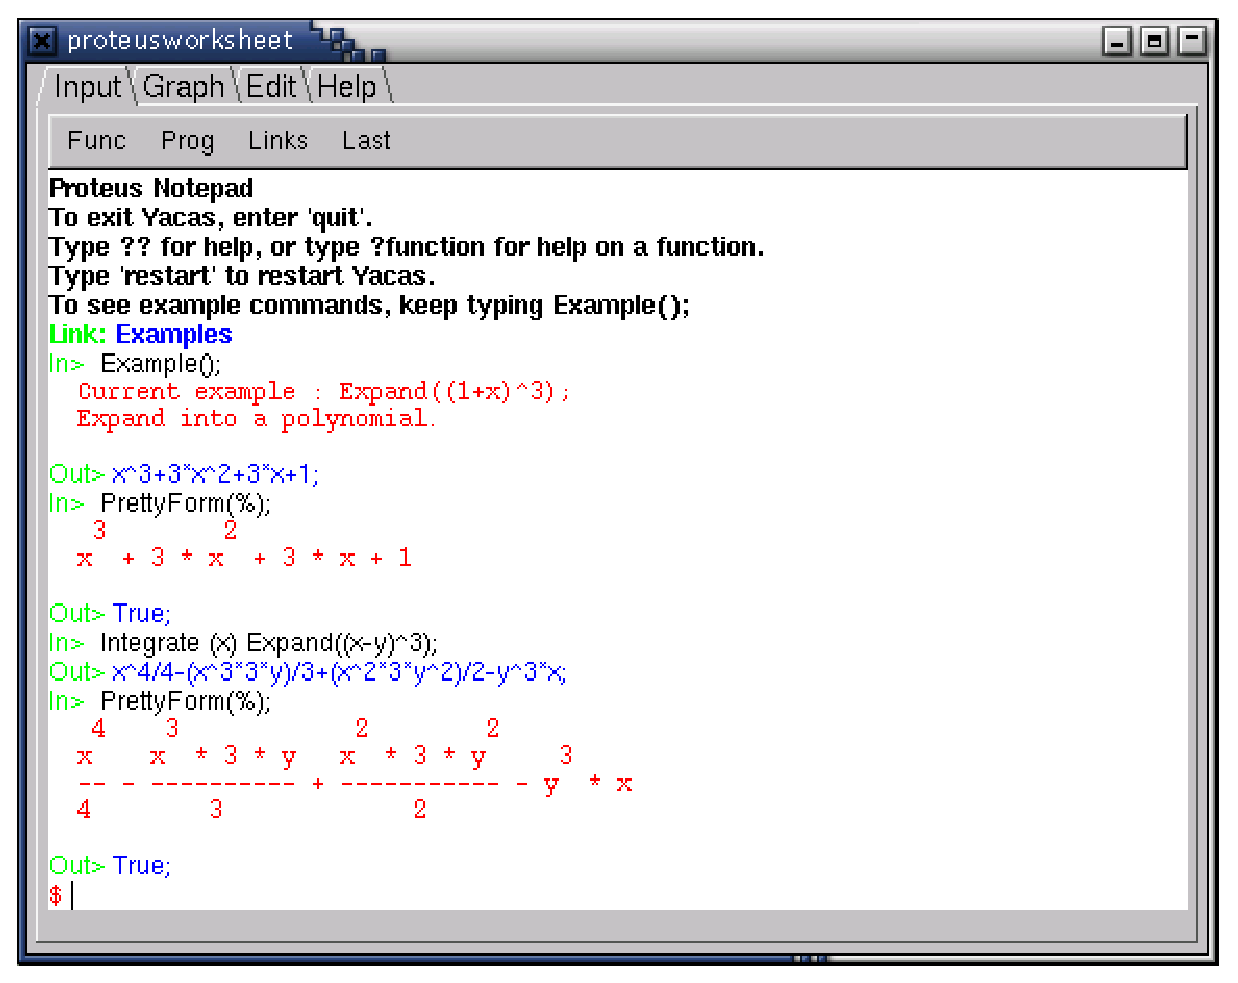
\includegraphics[width=\textwidth]{imagenes/proteus.eps}
\index{proteus}
\index{Yacas!proteus}
\caption{Proteus, interfaz gráfica para Yacas}
\end{figure}

La última línea (\verb+In>+) es el prompt de entrada de Yacas, que nos
indica que  el intérprete está  esperando nuestras órdenes.  Todas las
órdenes de Yacas deben terminar con un punto y coma (\verb+;+), aunque
el intérprete suele  añadirlo si no lo ponemos. Sin  embargo a la hora
de programar en  Yacas veremos que el punto y  coma hay que escribirlo
siempre,  de modo  que es  mejor acostumbrarse  a ponerlo  para evitar
posteriores dolores de cabeza.

Para ir abriendo  el apetito sigue la sugerencia de  Yacas: ejecuta la
función  \verb+Example();+ varias  veces. Por  supuesto no  tienes que
teclear el comando todas las veces, ya que Yacas cuenta con edición de
línea. Esto  incluye que todos los  comandos que ejecutes en  Yacas se
almacenarán  en un  historial, y  para repetirlos  puedes recuperarlos
pulsando  la  tecla  de  cursor hacia  arriba.  Este  historial  queda
guardado en  el fichero \verb+~/.yacas_history+. Veamos  la salida que
produce Yacas tras varias ejecuciones de \verb+Example();+.

\begin{verbatim}
In> Example();
Current example : 40!;

Simple factorial of a number.

Out> 815915283247897734345611269596115894272000000000;
In> Example();
Current example : D(x)Sin(x);

Taking the derivative of a function (the derivative of Sin(x) with
respect to x in this case).

Out> Cos(x);
In> Example();
Current example : Taylor(x,0,5)Sin(x);

Expanding a function into a taylor series.

Out> x-x^3/6+x^5/120;
In> Example();
Current example : Integrate(x,a,b)Sin(x);

Integrate a function.

Out> Cos(a)-Cos(b);
In> Example();
Current example : Solve(a+x*y==z,x);

Solve a function for a variable.

Out> (z-a)/y;
In> Example();
Current example : Limit(x,0)Sin(x)/x;

Take a limit.

Out> 1;
\end{verbatim}

En cualquier momento puedes acceder  a la documentación de una función
ejecutando la función  precedida por un signo  de interrogación, p.ej.
\verb+?IsFreeOf+. Un detalle  importante de Yacas es  que, como muchos
lenguajes del mundo de Un*x, es sensible a las mayúsculas; esto es, no
es lo mismo \verb+esto+ que \verb+Esto+ ni que \verb+eSTO+.

Estos ejemplos ilustran  lo fácil que es obtener  buenos resultados en
cálculos  simbólicos  con  Yacas.  Sin  embargo  es  probable  que  el
resultado del siguiente ejemplo no te resulte fácil de interpretar:

\begin{verbatim}
In> Integrate(x) Expand((x-y)^3);
Out> x^4/4-(x^3*3*y)/3+(x^2*3*y^2)/2-y^3*x;
\end{verbatim}

la forma en  que Yacas recibe nuestra orden de  integrar $\int (x-y)^3
\, dx$ no es nada críptica, pero su respuesta no es precisamente fácil
de  leer. Esta  forma de  mostrar  las expresiones  matemáticas es  la
normal  en  Yacas,  pero  no  la única.  Podemos  pedir  a  Yacas  que
muestre  las  expresiones  de  forma más  ``bonita''  con  la  función
\verb+PrettyForm()+.

\index{Yacas!PrettyFrom}

\begin{verbatim}
In> PrettyForm(%)

 4    3            2        2         
x    x  * 3 * y   x  * 3 * y     3    
-- - ---------- + ----------- - y  * x
4        3             2              

Out> True;
\end{verbatim}

El signo \verb+%+ es una referencia que apunta siempre al último valor
devuelto por el intérprete, es decir  lo que aparezca a la derecha del
último \verb+Out>+. Esta referencia sólo está disponible cuando usamos
Yacas  como intérprete  interactivo,  no se  puede  utilizar desde  un
script.

Otras  formas  de mostrar  una  expresión  son  las utilizadas  en  el
lenguaje  de  programación  C  y  en  el  lenguaje  tipográfico  \TeX.
Para  mostrar  una  expresión  de estas  formas  están  las  funciones
\verb+CForm()+  y \verb+TeXForm()+  respectivamente. Fíjate  que estas
funciones  no devuelven  la  expresión  que muestran,  por  lo que  no
podemos  utilizar  la  referencia  \verb+%+ dos  veces  seguidas  para
mostrar  una  expresión  (la  segunda mostraría  la  expresión  lógica
\verb+True+). Por  eso escribimos  \verb+Integrate(x) Expand((x-y)^3)+
en cada línea:

\index{Yacas!CFrom}
\index{Yacas!TeXFrom}

\begin{verbatim}
In> CForm (Integrate(x) Expand((x-y)^3))
Out> "pow(x, 4.) / 4. - ( pow(x, 3.) * 3. * y)  / 3. + ( pow(x, 2.) * 
3. * pow(y, 2.))  / 2. - pow(y, 3.) * x";
In> TeXForm (Integrate(x) Expand((x-y)^3))
Out> "$\frac{x ^{4}}{4}  - \frac{x ^{3} 3 y}{3}  + \frac{x ^{2} 3 y ^{
2}}{2} - y ^{3} x$";
\end{verbatim}

La función \verb+CForm()+ devuelve la expresión escrita en lenguaje C,
de forma que  podemos incluirla en el  código de un programa  en C. La
función \verb+TeXForm()+ devuelve la  expresión escrita en el lenguaje
tipográfico  \TeX, de  forma  que podemos  incluirla  en un  documento
escrito en  \TeX~ o \LaTeX.  Por ejemplo,  este libro está  escrito en
\LaTeX, lo  que me  permite incluir la  salida de  \verb+TeXForm()+ en
este  mismo párrafo  con  sólo copiar  y pegar.  De  esta forma  puedo
escribir: $$\int  (x-y)^3 \, dx  = \frac{x  ^{4}}{4} - \frac{x  ^{3} 3
y}{3} + \frac{x ^{2} 3 y ^{2}}{2} - y ^{3} x$$

En ocasiones nos  interesa conocer el valor numérico  de una expresión
determinada, y posiblemente sólo nos interese un número determinado de
decimales.  Yacas  es un  lenguaje  de  precisión arbitraria,  lo  que
significa que puedes  pedirle toda la precisión que  quieras, pero ten
cuidado no le pidas demasiada precisión  si tu máquina no es realmente
potente.

La función \verb+Precision()+ establece  el número de cifras decimales
con  las  que se  aproximarán  los  valores. Estas  aproximaciones  se
realizan con  la función  \verb+N()+, que  además permite  saltarse la
precisión establecida por \verb+Precision()+ pasándosela como segundo
parámetro. En el siguiente ejemplo se ilustra esto:

\index{Yacas!presición}

\begin{verbatim}
In> alpha := Sqrt (Pi ())
Out> Sqrt(3.1415926535897932384626433832795028841971694);
In> Precision (2);
Out> True;
In> N (alpha)
Out> 1.77;
In> Precision (20);
Out> True;
In> N (alpha)
Out> 1.77245385090551602729;
In> N (alpha, 50)
Out> 1.77245385090551602729816748334114518279754945629866;
\end{verbatim}

Normalmente  no hay  problema  por  pedirle a  Yacas  unos cientos  de
dígitos de precisión, pero siempre que  vayas a trabajar con números o
precisiones enormes recuerda que el tiempo necesario para los cálculos
aumentará rápidamente.



\section{Variables y funciones}

\index{Yacas!variables}
\index{Yacas!funciones}

En Yacas se entiende por variable un objeto al que se puede asignar un
valor.  Las variables  pueden  llamarse como  quieras  siempre que  el
nombre  empiece  por  una  letra  y continúe  con  letras  y  números.
Para  asignar un  valor  a  una variable  se  utiliza  el operador  de
asignación \verb+:=+ en lugar de \verb+=+ (este último se utiliza como
comparador). En cualquier momento puedes  ver el valor de una variable
tecleando su nombre como si fuera  un comando de Yacas, y esto también
es válido en un script. Asignaciones válidas son:

\begin{verbatim}
In> n := 10;
Out> 10;
In> m := n!;
Out> 3628800;
In> n
Out> 10;
In> m
Out> 3628800;
\end{verbatim}

Si en algún momento quieres que una variable pierda su valor no tienes
más que ``limpiarla'' con la función \verb+Clear()+:

\begin{verbatim}
In> m
Out> 3628800;
In> Clear (m);
Out> True;
In> m
Out> m;
\end{verbatim}

Las funciones  son como las  variables, con  el añadido de  que pueden
depender de una o más  variables. Además con Yacas podemos sobrecargar
una función, esto  es, definir dos funciones con el  mismo nombre pero
distinto número de  variables de forma que se evalúe  una u otra según
el número de parámetros que reciba.

Como ejemplo definimos la función \verb+Area+ de dos formas: si recibe
un parámetro  devuelve el área  del círculo con  el radio igual  a ese
parámetro, pero si recibe dos parámetros devuelve el área de la elipse
que tenga esos dos parámetros como radios.

\begin{verbatim}
In> Area (r) := Pi () * r^2;
Out> True;
In> Area (a, b) := Pi () * a * b;
Out> True;
In> Area (3);
Out> 28.2743338823;
In> Area (3, 5);
Out> 47.1238898035;
\end{verbatim}

Al definir  una función, Yacas no  evalúa la parte de  la derecha sino
que se asigna  como expresión simbólica. Esto puede  no interesarte en
casos como el que ilustra el siguiente ejemplo:

\begin{verbatim}
In> f(x) := x^5;
Out> True;
In> g(x) := D(x) f(x);
Out> True;
In> g(x)
Out> 5*x^4;
In> g(2)
Out> 5*x^4;
\end{verbatim}

Sería  deseable que  \verb+g(2)+  devolviera el  valor  de la  función
\verb+g(x)+  cuando  \verb+x+  vale  $2$,   pero  no  lo  hace  porque
\verb+g(x)+ almacena la expresión  \verb+5*x^4+ sin ninguna referencia
a la  necesidad de evaluarla en  un valor determinado. Sin  embargo si
indicamos a  Yacas que  evalúe la  expresión antes  de asignarla  a la
función  (mediante  \verb+Eval()+)  podremos  pedirle  que  evalúe  la
función \verb+g(x)+ en valores determinados. Esto que parece un follón
es  en realidad  simple, el  siguiente ejemplo  muestra el  código que
funciona como es de esperar:

\begin{verbatim}
In> g(x) := Eval (D(x) f(x));
Out> True;
In> g(x)
Out> 5*x^4;
In> g(2)
Out> 80;
\end{verbatim}



\section{Listas}

\index{Yacas!listas}

Uno de  los elementos más  importantes del  lenguaje de Yacas  son las
listas, que como era de esperar son grupos de objetos ordenados. Yacas
representa las listas  con sus elementos entre llaves  y separados por
comas.  Los  vectores  son  listas,  y  las  matrices  son  listas  de
listas. De  hecho, cualquier expresión  matemática en Yacas  puede ser
transformada en una  lista. Para acceder a los elementos  de una lista
puedes  usar la  notación habitual  en los  corchetes, y  no sólo  con
números  sino también  con secuencias  de ellos.  Los elementos  de la
lista pueden ser cualquier tipo de objetos.

\begin{verbatim}
In> lista := {a, b, c, d, e, f};
Out> {a,b,c,d,e,f};
In> lista[2];
Out> b;
In> lista[2 .. 4];
Out> {b,c,d};
\end{verbatim}

Fíjate  que los  espacios a  ambos  lados del  operador \verb+..+  son
necesarios  para distinguir  estos puntos  de los  que podrían  formar
parte de un número.

También puedes  indexar una lista  con palabras, no sólo  con números.
Esto  te permite  tener pequeñas  bases de  datos en  forma de  listas
asociativas con parejas clave -- valor.

\begin{verbatim}
In> boy := {};
Out> {};
In> boy["nombre"] := "Eric";
Out> True;
In> boy["apellido"] := "Cartman";
Out> True;
In> boy["edad"] := 7.34;
Out> True;
In> boy["educado"] := False;
Out> True;
In> boy
Out> {{"educado",False},{"edad",7.34},{"apellido","Cartman"},
{"nombre","Eric"}};
\end{verbatim}



\section{Álgebra Lineal}

\index{Yacas!Álgegra Lineal}
\index{Yacas!matrices}
\index{Yacas!vectores}

Los  vectores  de  dimensión  fija  se  representan  mediante  listas.
La  lista  \verb+{1,2,3}+ es  el  vector  $(1,2,3)$. Las  matrices  se
representan  como vectores  de  vectores. Dado  que  los vectores  son
realmente listas, sus elementos pueden  asignarse igual que los de las
listas:

\begin{verbatim}
In> l := ZeroVector (3);
Out> {0,0,0};
In> l;
Out> {0,0,0};
In> l[2] := 2;
Out> True;
In> l;
Out> {0,2,0};
\end{verbatim}

Yacas puede multiplicar vectores, matrices y números del modo usual en
álgebra lineal:

\begin{verbatim}

In> v := {1, 0, 0, 0}
Out> {1,0,0,0};
In> E4 := { {0, u1, 0,  0}, \
In>         {d0, 0, u2, 0}, \
In>         {0, d1, 0,  0}, \
In>         {0, 0,  d2, 0} }
Out> {{0,u1,0,0},{d0,0,u2,0},{0,d1,0,0},{0,0,d2,0}};
In> PrettyForm (%)

/                             \
| ( 0 )  ( u1 ) ( 0 )  ( 0 )  |
|                             |
| ( d0 ) ( 0 )  ( u2 ) ( 0 )  |
|                             |
| ( 0 )  ( d1 ) ( 0 )  ( 0 )  |
|                             |
| ( 0 )  ( 0 )  ( d2 ) ( 0 )  |
\                             /

Out> True;
In> CharacteristicEquation (E4, x)
Out> x^4-x*u2*d1*x-u1*d0*x^2;
In> Expand (%, x)
Out> x^4-(u2*d1+u1*d0)*x^2;
In> PrettyForm (%)

 4                            2
x  - ( u2 * d1 + u1 * d0 ) * x 

Out> True;
In> v  +  E4 * v  +  E4 * E4 * v  +  E4 * E4 * E4 * v
Out> {u1*d0+1,d0+(d0*u1+u2*d1)*d0,d1*d0,d2*d1*d0};
In> PrettyForm (%)

/                                 \
| u1 * d0 + 1                     |
|                                 |
| d0 + ( d0 * u1 + u2 * d1 ) * d0 |
|                                 |
| d1 * d0                         |
|                                 |
| d2 * d1 * d0                    |
\                                 /

Out> True;
\end{verbatim}

La librería estándar de Yacas incluye también cálculo del determinante
y  la inversa  de una  matriz,  autovectores y  autovalores (en  casos
simples) y resolución de sistemas  de ecuaciones lineales del tipo $Ax
= b$ donde $A$ es una matriz y $x$ y $b$ son vectores.



\section{Control de flujo}

\index{Yacas!control de flujo}

El lenguaje de  Yacas incluye algunas construcciones  y funciones para
el control  de flujo. Para ello  necesitas saber también que  Yacas te
permite agrupar bloques  de instrucciones de forma  que aparezcan como
una sola instrucción. Para ello simplemente encierra las instrucciones
del  bloque entre  corchetes  (\verb+[+ y  \verb+]+),  o bien  utiliza
la  función \verb+Prog()+  pasándole las  instrucciones separadas  por
\verb+;+.

Para  los  bucles  disponemos  de  las  funciones  \verb+ForEach()+  y
\verb+While()+. La  función \verb+ForEach (x, list) body+  ejecuta  el
bloque de  instrucciones \verb+body+  para cada  elemento de  la lista
\verb+list+ asignando el valor de cada elemento a la variable \verb+x+
en cada interación. La función \verb+While (predicate) body+ repite el
bloque \verb+body+  hasta que  la condición  \verb+predicate+ devuelva
\verb+False+.

Para   los  condicionales   está  la   función  
\verb+If (predicate, body1, body2)+,
en la  que  se  ejecuta  el bloque  \verb+body1+  si
\verb+predicate+ devuelve \verb+True+ o ejecuta el bloque \verb+body2+
si \verb+predicate+  devuelve \verb+False+, y en  ambos casos devuelve
el  valor devuelto  por  el  bloque ejecutado.  El  segundo bloque  es
opcional.  Si  llamas  a  \verb+If (predicate,  body1)+  se  ejecutará
el  bloque \verb+body1+  si  \verb+predicate+  devuelve \verb+True+  y
devolverá  el valor  que devuelva  \verb+body1+, o  bien se  devolverá
\verb+False+ si así lo hace \verb+predicate+.

Como ejemplo de control de flujo construimos una lista con los números
enteros pares  de $2$ a  $20$ y calculamos el  producto de los  que no
sean divisibles por $3$. Luego definimos  el factorial de un número de
forma recursiva.

\begin{verbatim}
In> L := {};
Out> {};
In> i := 2;
Out> 2;
In> While (i <= 20) [ \
In>   L := Append (L, i); \
In>   i := i + 2; \
In> ];
Out> True;
In> L;
Out> {2,4,6,8,10,12,14,16,18,20};
In> answer := 1;
Out> 1;
In> ForEach (i, L) [ \
In>   If ( Mod (i, 3) != 0, \
In>     answer := answer * i \
In>   ); \
In> ];
Out> True;
In> answer;
Out> 2867200;
In> Factorial (x) := [ \
In>   If ( IsInteger (x) And x >= 0, \
In>     If (x = 0, 1, \
In>       x * Eval (Factorial (x-1)) ), \
In>   False ); \
In> ];
In> Factorial (5)
Out> 120;
In> Factorial (25)
Out> 15511210043330985984000000;
\end{verbatim}

Una  barra  invertida  \verb+\+  al  final  de  una  línea  indica  al
intérprete de Yacas que la línea  no está terminada, sino que continúa
después  del salto  de carro.  En  este ejemplo  hemos utilizado  esto
descaradamente. Esto se puede utilizar en el intérprete para hacer que
nuestros comandos  sean más cómodos de  leer, pero no es  necesario al
escribir un script.



\section{Gráficas}

\index{Yacas!gráficas}

Yacas incorpora la posibilidad de representar gráficas bidimensionales
utilizando  GNUplot, si  bien  esta capacidad  depende  de que  tengas
instalado también  el programa  GNUplot. Para saber  si tu  versión de
Yacas  tiene soporte  para  GNUplot  fíjate en  la  primera línea  que
imprime el  intérprete cuando arranca, si  aparece \verb+[gnuplot.ys]+
es   que   tu   versión   de   Yacas   soporte   para   gráficas   con
GNUplot\footnote{Esto  era cierto  hasta la  versión 1.0.50  de Yacas,
pero  en el  momento de  escribir esta  nota la  versión 1.0.51  de mi
máquina no  aparece {\tt [gnuplot.ys]}  pero puede hacer  las gráficas
con la función {\tt Plot2D}}.

\begin{verbatim}
$ yacas
[editvi.ys] [gnuplot.ys] [unix.ys]
\end{verbatim}

La función para  representar gráficas es \verb+Plot2D()+  y recibe dos
parámetros: la expresión  (o lista de expresiones)  para representar y
el  intervalo  de  la  variable  en  la  forma  {\tt  valor\_minimo  :
valor\_maximo}.

En anteriores versiones de Yacas, la función para representar gráficas
era \verb+GnuPlot()+ y  recibía cuatro parámetros: el  valor mínimo de
la  variable, el  valor máximo  de la  variable, el  número de  puntos
utilizados para la representación y la función para representar. 

En los  siguientes ejemplos  calculamos el el  polinomio de  Taylor de
orden 5 para la función $\sin(x)$  en el origen y la representamos (en
rojo) junto con la función $\sin(x)$ (en verde).

\begin{figura}{yacas_gnuplot}{0.8}
\caption{Representación gráfica con GNUplot desde Yacas}
\end{figura}

\begin{verbatim}
In> f(x) := Eval (Taylor (x, 0, 5) Sin(x) )
Out> True;
In> Plot2D ({f(x), Sin (x)}, -Pi:Pi)
Out> True;
In> GnuPlot (-Pi(), Pi(), 50, {f(x), Sin(x)})
GnuPlot: created file gnuplot.tmp/gnudata.in1
GnuPlot: created file gnuplot.tmp/gnudata.in2
Out> True;
\end{verbatim}

\section{Programando con Yacas}

\index{Yacas!programación}

Si bien  el intérprete de  Yacas proporciona una interfaz  cómoda para
ejecutar  cálculos, cuando  éstos  se complican  resulta más  práctico
escribir un ``script'' y ejecutarlo  con Yacas. Para hacer un programa
con Yacas escribe en un fichero  la secuencia de comandos que componen
el  programa, incluyendo  definiciones de  funciones. Los  ficheros de
script  de Yacas  suelen tener  tener la  extensión {\tt  .ys} (no  es
obligatorio).  

Para ejecutar  el script simplemente  ejecuta Yacas dándole  el nombre
del fichero como parámetro. La opción {\tt -c} del comando {\tt yacas}
hace que Yacas  no muestre los prompts \verb+In>+  y \verb+Out>+ (útil
para sesiones no interactivas, como el caso de ejecutar un script). El
siguiente ejemplo  muestra como ejecutar  un script en Yacas,  en este
caso el script es el fichero de ejemplo {\tt lagrange.ys}

\begin{verbatim}
$ yacas -c lagrange.ys
\end{verbatim}

\begin{ejemplo}{lagrange.ys}{Script en Yacas que interpola una función}
\index{Yacas!script}
Script en Yacas  que muestra un interpolante de Lagrage  para una nube
de cinco  puntos tomados  de la función  $f(x) =  \frac{1}{1+x^2}$. En
este  ejemplo el  interpolante de  Lagrange  no es  el adecuado,  pero
nuestra intención  no es interpolar  $f(x)$
\end{ejemplo}

Otra   forma  de   ejecutar  un   script  es   desde  el   intérprete,
mediante  las  funciones  \verb+Load()+  y  \verb+Use()+.  La  función
\verb+Load("script.ys")+  lee  el  fichero \verb+script.ys+  y  evalúa
todas  las   expresiones  que   encuentre  en  él.   Siempre  devuelve
\verb+True+.  \verb+Use()+  hace lo  mismo  que  \verb+Load()+ con  la
salvedad de que sólo lee el fichero si no ha sido leído antes por otra
llamada \verb+Load()+ o \verb+Use()+.

Un uso  común de \verb+Use()+ es  cargar un fichero con  funciones con
las que queremos trabajar desde el  intérprete, de modo que no tenemos
que teclear  las funciones  cada vez  ni tampoco  hay que  ejecutar el
script. La función \verb+Load()+ resulta  útil para ejecutar un script
desde el  intérprete cuando queremos hacerlo  varias veces modificando
el script sin salir del intérprete.



\section{Un ejemplo real}

\index{Yacas!ejemplo real}

A continuación  explicamos un ejemplo  del uso  de Yacas ``en  la vida
real'': calcular la sucesión de Sturm  asociada a un polinomio real de
una variable  real. Esta sucesión  se utiliza  en el teorema  de Sturm
para  calcular el  número  de  raíces reales  de  un  polinomio en  un
intervalo de la  recta real. El algoritmo para  calcular esta sucesión
de polinomios no es complicado, pero  por si no lo conoces aquí tienes
una breve explicación:

El algoritmo  de Sturm parte  de un polinomio con  coeficientes reales
$p(x)$  y su  derivada $p'(x)$.  Tomando $f_0(x)  = p(x)$  como primer
polinomio  y $f_1(x)  =  p'(x)$ como  segundo  polinomio, se  realizan
sucesivas divisiones euclídeas utilizando  en cada división el divisor
de la  anterior como dividendo y  el opuesto del resto  de la anterior
como divisor. Al  cabo de un número finito de  iteraciones, en las que
$f_j(x)$ es el resto de la división $j-1$, se obtiene un resto nulo en
la iteración $m+1$.

\begin{eqnarray*}
f_0(x) & = & f_1(x) q_1(x) - f_2(x)          \\
f_1(x) & = & f_2(x) q_2(x) - f_3(x)          \\
& \vdots &                                   \\
f_{m-2}(x) & = & f_{m-1}(x) q_1(x) - f_m(x)  \\
f_{m-1}(x) & = & f_m(x) q_m(x)
\end{eqnarray*}

A  partir de  los polinomios  $f_j$ obtenidos  en estas  divisiones se
construye la sucesión de Sturm asociada a $p(x)$, que viene dada por

$$\left\{\hat{f}_j(x) = \frac{f_j(x)}{f_m(x)}\right\}_{j=0}^{n}$$

El teorema  de Sturm garantiza que  el número de raíces  del polinomio
$p(x)$ en  el intervalo  $[a,b]$ es exactamente  $V(a) -  V(b)$, donde
$V(x_0)$ es el número de variaciones  de la sucesión de Sturm evaluada
en el punto $x_0$,  i.e. el número de cambios de  signo en la suceción
$\left\{   \hat{f}_0(x_0),   \hat{f}_1(x_0),  \ldots,   \hat{f}_m(x_0)
\right\}$.

Para implementar esto en Yacas definimos la función \verb+Sturm()+ que
recibe el polinomio \verb+P+ junto con la variable en la que éste está
expresado \verb+x+  y genera una  lista \verb+L+ con el  polinomio, su
derivada  y los  sucesivos restos  de las  divisiones euclídeas.  Para
ahorrar esfuerzo  computacional acotamos el  número de términos  de la
lista con el grado del polinomio \verb+P(x)+, ya que éste es el número
máximo de divisiones necesarias para encontrar el máximo común divisor
del polinomio y  su derivada. Luego busca el último  polinomio no nulo
en  \verb+L+, que  es  el  máximo común  divisor  del  polinomio y  su
derivada, y construye la sucesión de Sturm en una nueva lista \verb+S+
que  finalmente devuelve  como  valor  de retorno  de  la función.  La
función \verb+Simplify+ simplifica cualquier expresión que reciba.

\begin{ejemplo}{sturm.ys}{Script en Yacas que implementa el algoritmo de Sturm}
Script en Yacas que implementa el algoritmo de Sturm.
\end{ejemplo}

En  el  script  escribimos  esta   función  y  añadimos  los  comandos
necesarios  para  ejecutar  un test.  La  función  \verb+RandomPoly()+
genera un  polinomio aleatorio, lo mostramos  con \verb+PrettyForm()+,
calculamos su sucesión de Sturm y la mostramos con \verb+PrettyForm()+
de nuevo. El resultado de ejecutar el script es el siguiente:

\begin{verbatim}
     3         2            
7 * x  + 10 * x  + 3 * x + 3


/                                          \
|     /           2                      \ |
| 9 * \ -96605 * x  + 73253 * x - 181452 / |
| ---------------------------------------- |
|                 2685619                  |
|                                          |
| 81 * ( -139 * x - 117 )                  |
| -----------------------                  |
|          19321                           |
|                                          |
| 1                                        |
\                                          /
\end{verbatim}

Este ejemplo  real ha sido  extraido del programa presentado  por unos
alumnos como trabajo para  asignatura ``Álgebra Computacional'' que se
imparte en la Facultad de Matemáticas  de la Universidad de La Laguna.
En  teoría  debieron realizar  el  trabajo  utilizando Maple  V,  pero
propusieron al profesor la alternativa  de programarlo en Yacas y éste
aceptó con  curiosidad. El programa  aproxima las raíces reales  de un
polinomio utilizando el  algoritmo de Sturm para aislar  las raíces en
intervalos y aproximándolas  con el método de la  bisección (raíces de
multiplicidad  impar)  o  con  el método  de  cristalización  simulada
(raíces de multiplicidad par). El trabajo fue expuesto en clase y tuvo
la calificación de sobresaliente, el código y las transparencias están
disponibles en {\tt http://www.fmat.ull.es/\~{}miguev/algcomp/}

